\documentclass[12pt, a4paper]{article}
\usepackage{a4wide}
\usepackage{anysize}
\usepackage[centertags]{amsmath}
\usepackage{amsfonts,amssymb,amsthm}
\usepackage{graphicx}
\usepackage{natbib}
\usepackage{wrapfig}
\usepackage{iitbieortitle}

\usepackage{mathptmx}
\usepackage{alphalph}
\def\theequation{\AlphAlph{\value{equation}}}


% \usepackage{fontspec}
% \setmainfont[Ligatures=TeX]{Times New Roman.ttf}
%\usepackage{fullpage}
%\usepackage{rotating}

\renewcommand{\baselinestretch}{1.15} %line spacing
\marginsize{1in}{1in}{1in}{1in}   %left right top bottom
%\textwidth 6in
% Title Page

\begin{document}

\pagenumbering{roman}
\pagestyle{plain}
\def\title{CS 403: Algorithm Design and Analysis }
\def\who{\LARGE IIT Mandi}
\def\guide{}
 %\href{mailto:deepanshu3131@gmail.com}{\custombold{Deepanshu Sapra}}

\titlpage
\tableofcontents



\newpage
\pagenumbering{arabic}


\section{Objective}
This report tend to analyse the algorithm made for solving given programming problems.\\
The problem statement is as follows: \\A) Write a program to accept an integer n$>$ 0, and generate all permutations between 1 to n.\\
\\B) Write a program to accept a set of n elements, and generate all the subsets of that set. Assume that all elements of the set are characters.\\
\section{Methodology}
\subsection{Part-\RNum{A}}
There are n! possible permutations of n. I have made an array of size n and generated its permutation by swapping its starting index and working index then recursively calculating permutation of rest of array and checked if starting index is equal to ending index then printing the generated array and then backtracked it to original array recursively. I have taken value of n from 1 to 13 as it was taking too much time for n $>$ 13. Since I am generating every permutation and printing it so the Asymptotic complexity is $\mathcal{O}(nn!)$.
\begin{center}
 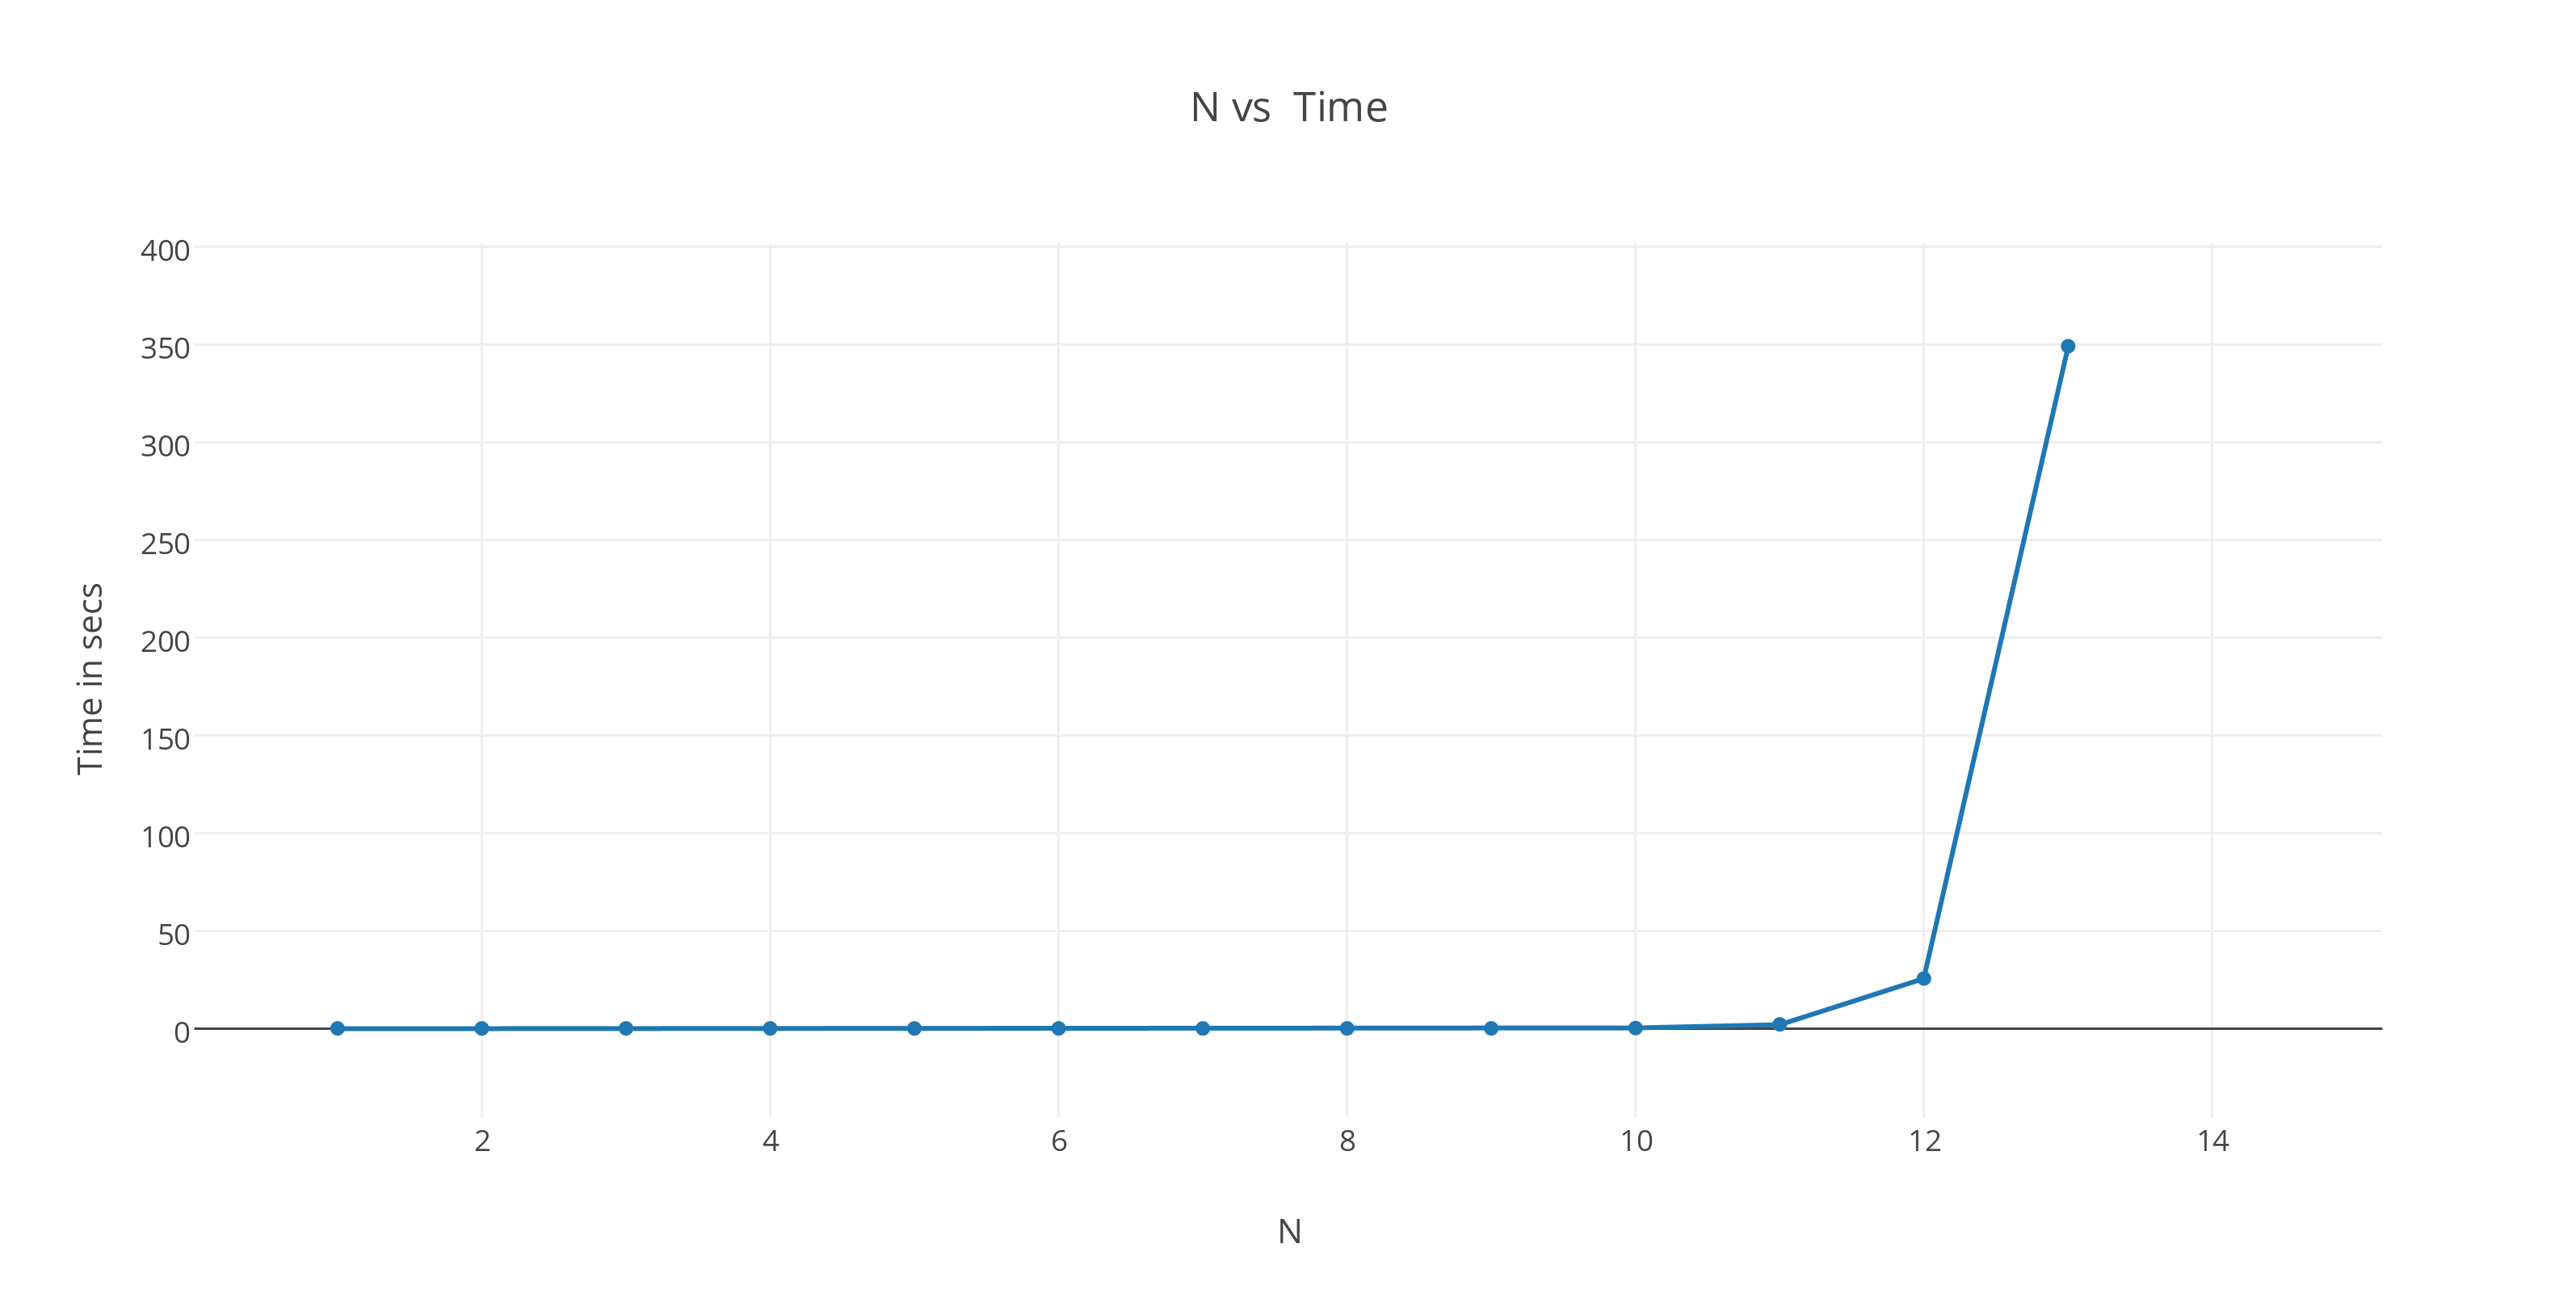
\includegraphics[height = 10cm, width = 16cm]{PartA.png}
\end{center}
\subsection{Part-\RNum{B}}
There are $2^{n}$ possible subset of given set. First I have calculated the size of power set using algorithm of Asymptotic complexity $\mathcal{O}(\log{}n)$  the for each element in power set I have generated the corresponding set element. I have taken length of string ranging from 1 to 30 as it was taking too much time for length $>$ 30. Since I am generating every 
and in part B the Asymptotic complexity is of order n$2^{n}$ i.e O(n$2^{n}$).\\
%%%%%%%%%%%%%%%%%%%%%%%fig:2%%%%%%%%%%%%%%%%%%%%%%%%%%
\begin{center}
 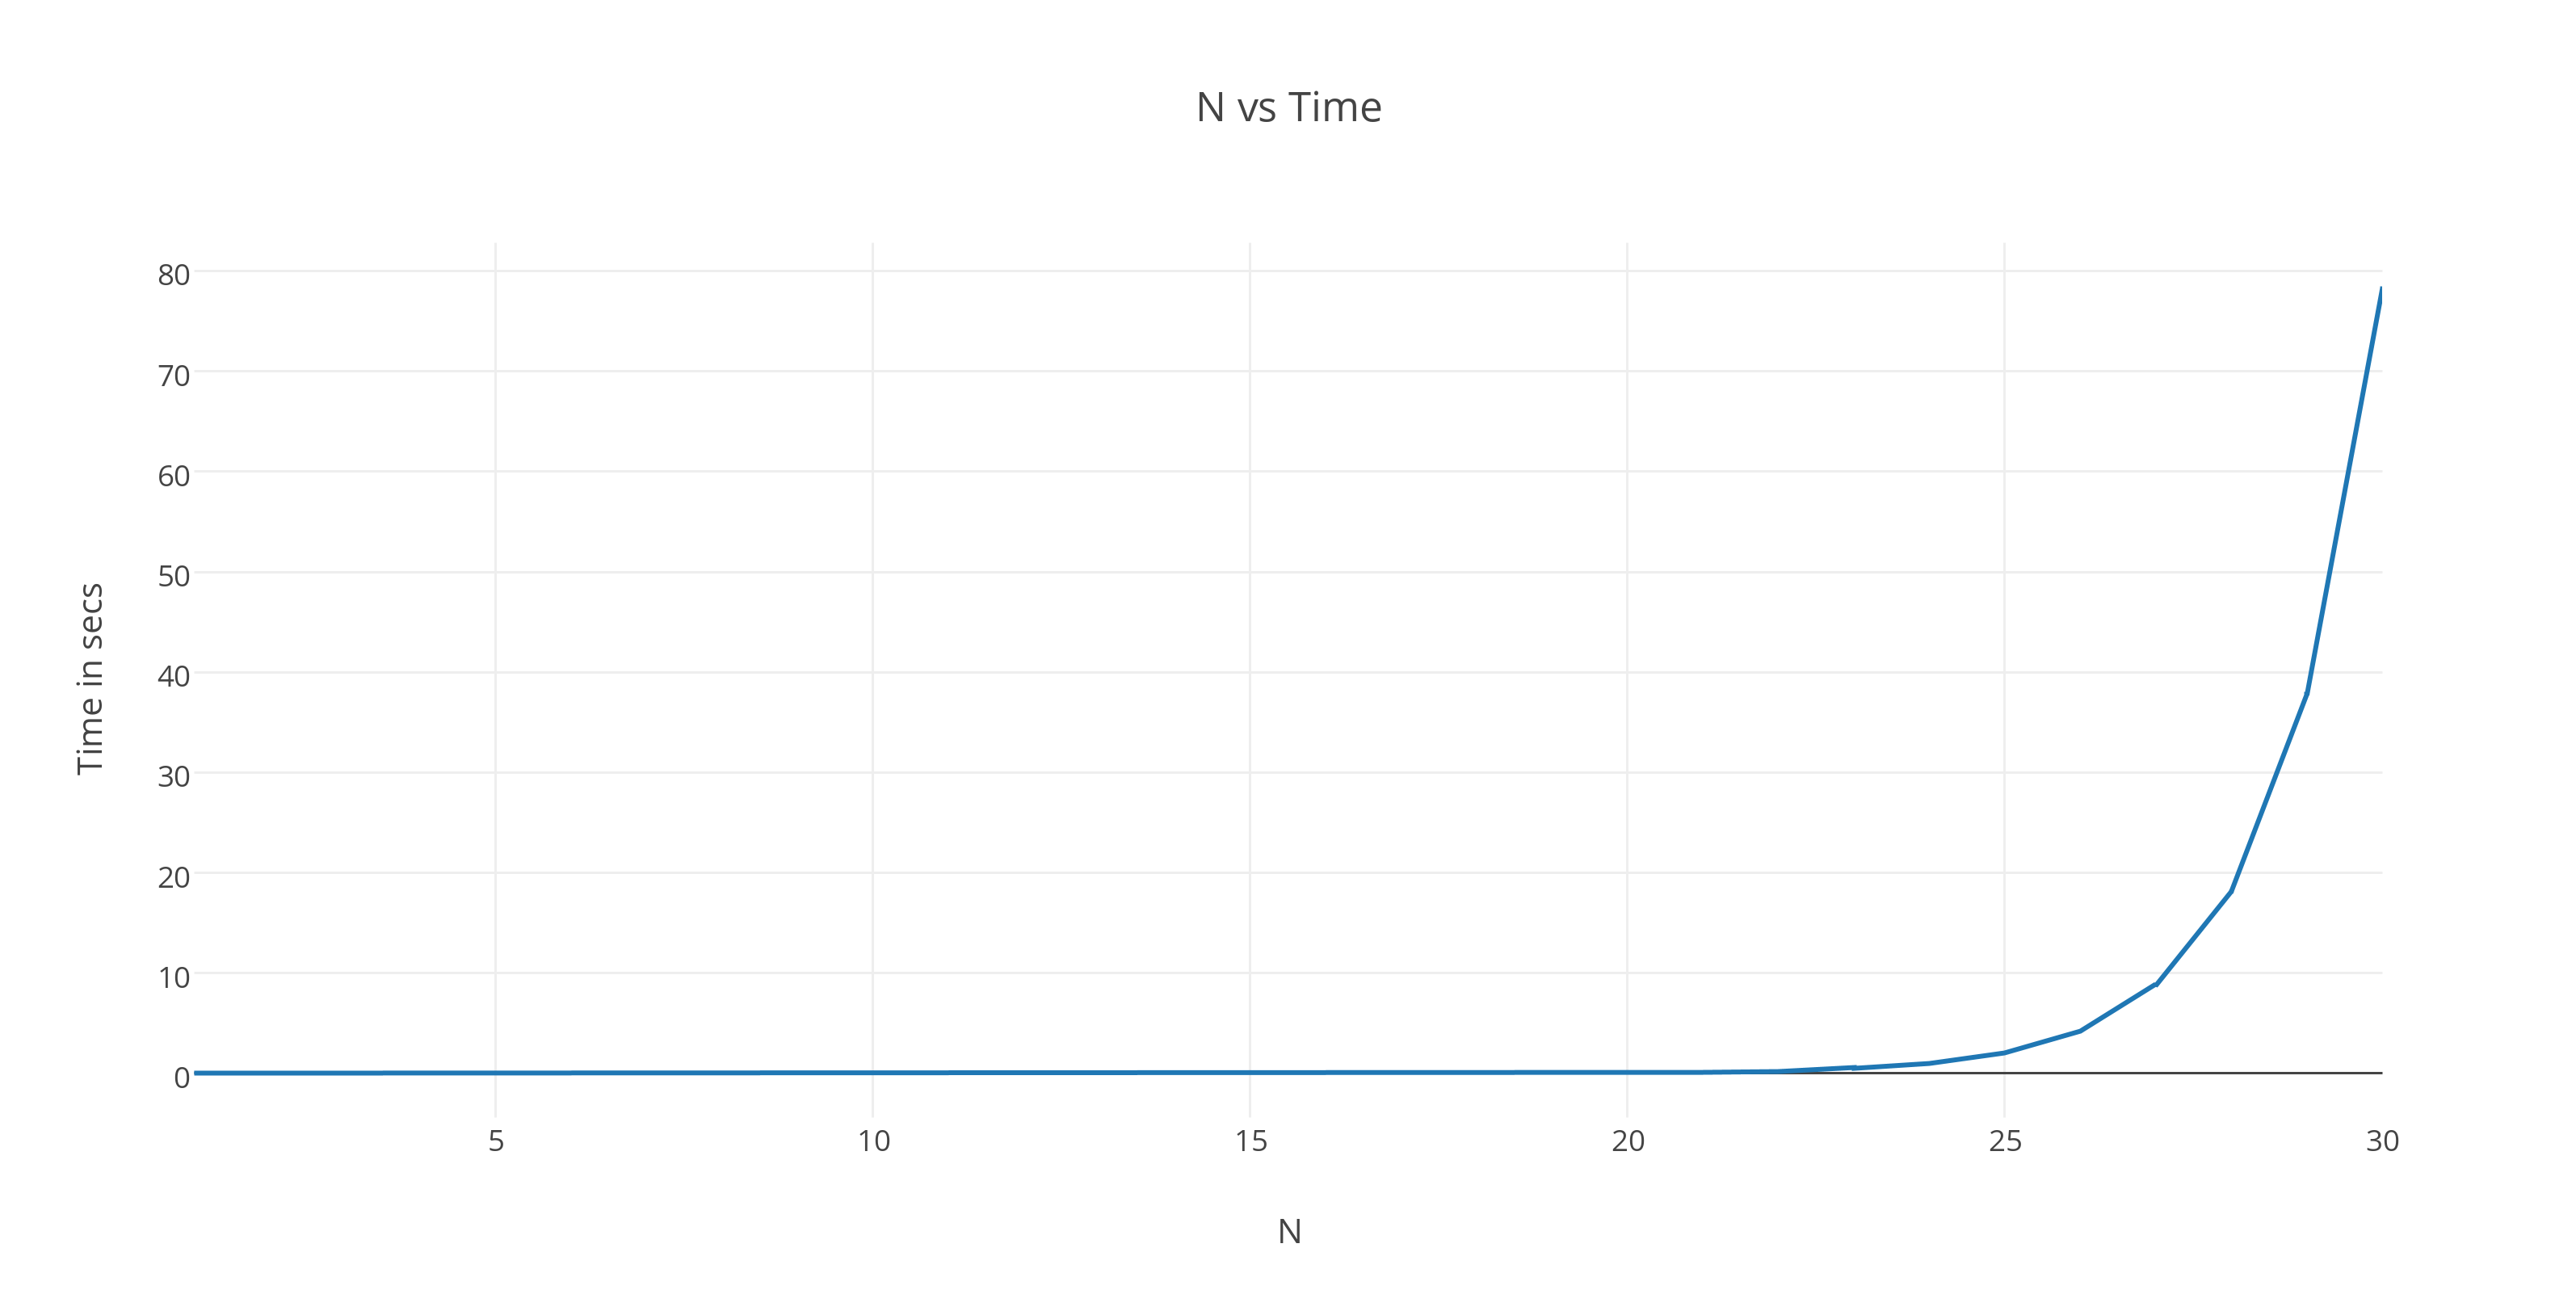
\includegraphics[height = 10cm, width = 16cm]{PartB.png}
\end{center}


%%
\newpage
\section{Conclusions}



%\bibliographystyle{elsart-harv}
%\bibliographystyle{amsplain}
%\bibliography{EwoRefer}

\end{document}          
